\documentclass[a4paper,11pt]{article}


%for coloring cell in a table
\usepackage[table]{xcolor}% http://ctan.org/pkg/xcolor

\usepackage{amsmath}
\usepackage{amssymb}

% for proofs  environment
\usepackage{amsthm}

% for 3d plots
\usepackage{pgfplots}
\usepackage{pgfplotstable}
\usepgfplotslibrary{patchplots}

\usepackage[backend=bibtex]{biblatex}
\bibliography{slides7}

% for probability trees
\usepackage{tikz}
\usetikzlibrary{trees}

% for Venn diagrams
\usetikzlibrary{shapes,backgrounds}

% for plots
\usepackage{ pgfplots}
% inserted on suggestion in warning during compilation
\pgfplotsset{compat=1.9}

%for strikethrough text
\usepackage{soul}

%for R source code listing
\usepackage{listings}

%for block quotes
\usepackage{csquotes}

\newtheorem{thm}{Theorem}
\newtheorem{lem}[thm]{Lemma}

% For not indenting the first line of paragraphs:
\setlength{\parindent}{0pt}
% define the title
\author{John Hancock}
\title{MIT Introduction to Statistics 18.05 Class 7 Slides - Solutions}
\begin{document}
% generates the title
\maketitle
% insert the table of contents
\tableofcontents
\section{References and License}
We are answering questions in the material from MIT OpenCourseWare
course 18.05, Introduction to Probability and Statistics.

In this document we are answering questions Orloff and Bloom ask in
\cite{slides7}.

Please see the references section for detailed citation information.

The material for the course is licensed under the terms at
\url{http://ocw.mit.edu/terms}.

We use documentation in  \cite{logicNot}, \cite{proofs}, \cite{bars},
\cite{packageClash}, \cite{curlyBrace}, \cite{cases} to write the \LaTeX source code for this document.

\section{Estimate Error}
The first question Orloff and Bloom ask in \cite{slides7} is about an
accountant that rounds his cacluations (entries) to the nearest dollar.  We
assume the accountant has made 300 calculations.  Orloff and Bloom want us
to estimate the probability that the total error is greater than five
dollars.

We use the central limit theorem \cite{reading6b} and techniques for estimating
probability that Orloff and Bloom show in \cite{reading6b} in order to find
this estimate.

In order to apply the central limit theorem, we first define a random variable
$X_i$.  $X_i$ is the error the accountant makes on her $i^th$ calculation.
Orloff and Bloom tell us that $X_i$ is uniformly distributed on
$\left[-0.5, 0.5 \right]$.

We also need the mean $\mu$, and standard deviation $\sigma$ of $X_i$ in order
to make our estimate.

In \cite{reading5c} Orloff and Bloom state that a uniformly distributed random
variable on $\left[a, b \right]$ has the distribution function
$f\left(x \right) = \frac{1}{a-b}$.

In \cite{reading6a} Orloff and Bloom define the mean $E\left(X \right)$ of a
continuous random variable $X$ with pdf $f\left(x \right)$ to be:

\begin{equation}
  E\left(X \right) = \int_a^b xf\left(x \right) \,dx
\end{equation}

For this problem, $f\left( x \right) = \frac{1}{-0.5 - 0.5} = -1$.  Therefore
we apply Orloff and Bloom's definition of the mean value of a continuous random
variable to find that the mean value of $X_i$ is

\begin{equation}
  E\left(X_i \right) = \int_{-0.5}^{0.5}-x \,dx.
\end{equation}

We use the power rule for integrals from \cite{basicInt} to find the antiderivative
of the function above that we must integrate in order to find the mean value of
$X_i$.  The antiderivative of $g\left( x \right) = -x$ is $\frac{-x^2}{2}$.

We replace the integral on the right hand side of the equation above with its
antiderivative:

\begin{equation}
  E\left(X_i \right) = \frac{-x^2}{2} \bigg\rvert_{-0.5}^{0.5}.
\end{equation}

And we evaluate the antiderivative over the interval $\left[-0.5, 0.5 \right]$:


\begin{equation}
  E\left(X_i \right) = \frac{-\left(-0.5^2 \right)}{2} - \frac{-\left(0.5^2 \right)}{2}
\end{equation}

Now we do some arithmetic to simplify the right hand side of the equation above:

\begin{equation}
  E\left(X_i \right) = \frac{-1}{8} - \frac{-1}{8} = 0.
\end{equation}

In order to find the standard deviation of $X_i$, we use a property of variance
from \cite{reading6a}, for a continuous random variable $X$:
\begin{equation}
\text{Var}\left(X \right) = E\left(X^2 \right) - E\left(X \right)^2.
\end{equation}

We apply the same reasoning to find $E\left(X_i^2 \right)$ that we use to find
$E\left(X_i \right)$:

\begin{equation}
  E\left(X_i^2 \right) = \int_{-0.5}^{0.5}- \left(x^2 \right) \,dx.
\end{equation}

This implies:

\begin{equation}
  E\left(X_i^2 \right) = \frac{-x^3}{3} \bigg\rvert_{-0.5}^{0.5}.
\end{equation}

Which implies

\begin{equation}
  E\left(X_i^2 \right) = \frac{-\left(-0.5^3 \right)}{3}
  - \frac{-\left(0.5^3 \right)}{3}
\end{equation}

The right hand side of the equation above simplifies to:

\begin{equation}
  E\left(X_i^2 \right) = \frac{-\left(-1 \right)}{24}
  - \frac{-1}{24}
\end{equation}

Therefore the variance of $X_i$ is $\frac{1}{12}$.

Orloff and Bloom ask us to estimate the probability of the size of the error the accountant
makes after 300 calculations.  So, we define a random variable $S$ to be the
sum of 300 values of the $X_i$. Therefore $S$ is the total erorr that the
accountant makes after 300 calculations.

In order use the central limit theorme to estimate the probability that a random
variable is in a range we need to know its mean and standard deviation.

Thereofre we need to know the mean of $S$.  We start with:

\begin{equation}
E\left(S \right) = E\left(\sum_{i=1}^n X_i \right).
\end{equation}

We use a property of expected value from \cite{reading6a} to find that the mean value
\begin{equation}
E\left(S \right) = \sum_{i=1}^300 E\left(X_i \right).
\end{equation}

Above we found that $E\left(X_i \right)=0$.  Therefore, by the equation above,
$E\left(S \right) = 0$. Mean and expected value are synonymous, and to use
the notation Orloff and Bloom use in their treatment of the central limit
theorem we write the mean of S, $\mu_s=0$.

Now we turn our attention to finding the variance and standard deviaion of $S$.

In \cite{reading6a} Orloff and Bloom state that the variance of the
sum of independent random varialbes is the sum of their variances. We assume the
collection of $X_i$ are independent.

This assumption allows us to write that the variance of $S$,
\begin{equation}
  \text{Var}\left(S \right) = \sum_{i=1}^300 \frac{1}{12} = 25.
\end{equation}

Becausee standard deviation is the square root of variance, the standard
deviation of $S$, $\sigma_S$ is 5.

Orloff and Bloom are asking us to compute the probability that the total error
the accountant makes after 300 calculations is more than $5\$$.  The total error
the accountant makes might be a positive or negative value, so we need to
estimate the probability that $S < -5\$$ or $S > 5$. However, this probability
is equal to $1 - P\left( -5 \leq S \leq 5 \right)$. We state this relationship
with the equation:
\begin{equation}\label{probEq}
  P\left(\left|S\right| < 5 \right) = 1 - P\left( -5 \leq S \leq 5 \right).
\end{equation}

The central limit theorem states that standardized $S$ approximately follows
the normal distribution $N\left( 0, 1 \right)$.

We standardize $S$, and apply the central limit theorem like Orloff and
Bloom do in \cite{reading6b} to get the approximation:

\begin{equation}
P \left( -5 \leq S \leq 5 \right)
=P \left( -\frac{5}{5} \leq \frac{S-\mu_S}{\sigma_S} \leq \frac{5}{5} \right)
=P \left( -1 \leq \frac{S-0}{5} \leq 1 \right)
  \approx P\left(-1 \leq Z > 1 \right)
\end{equation}

Note: the equations above are legal because $S$ is a continuous random
variable, and therefore we compute the eprobability that $S$ is in a given
interval with and integral. In the equations above we are using the
property of integration that states a constant times the integral of a function
is the integral of the constant times that function \cite{basicInt}.

The rule of thumb \cite{reading6b} tells us that
$P\left(-1 \leq Z \leq 1 \right) \approx 0.68$.  We use equation \ref{probEq} to
obtain our estimate that the probability that the total error the accountant
makes after 300 calculations is more than $5\$$ is 0.32.


\section{Difference of Dice}

The second question Orloff and Bloom have is on the discrete events.
Orloff and Bloom define two discrete random variables $X$, and $Y$.
$X$ and $Y$ are the values we roll using two six-sided dice.
They then define the event $A$ as the event where the difference
$Y-X$ is greater than or equal to 2.

The event $A$ is a set of outcomes.  Each member of $A$ is
an outcome of an event where we roll two dice, and the difference
between the value we roll with the first die, and the value
we roll with the second die is greter than or equal to 2.

We arrange the possible differences of $X$ and $Y$ in a table.

Thus, we represent all possible outcomes the event where we roll
two dice, and then subtracting the value we roll with the first die
from the value we roll with the second die as a cell in the
table below.

\begin{center}
  \begin{tabular}{ | c | c | c | c | c | c | c |}
    \hline
    $X/Y$ & 1  &  2 &  3 &  4 &  5 &  6   \\ \hline
    1     & 0  & -1 & -2 & -3 & -4 & -5   \\ \hline
    2     & 1  &  0 & -1 & -2 & -3 & -4   \\ \hline
    3     & \cellcolor{blue!25} 2  &  1 &  0 & -1 & -2 & -3   \\ \hline
    4     & \cellcolor{blue!25} 3  &  \cellcolor{blue!25} 2 &  1 &  0 & -1 & -2   \\ \hline
    5     & \cellcolor{blue!25} 4  &  \cellcolor{blue!25} 3 &  \cellcolor{blue!25} 2 &  1 &  0 & -1   \\ \hline
    6     & \cellcolor{blue!25} 5  &  \cellcolor{blue!25} 4 &  \cellcolor{blue!25} 3 &  \cellcolor{blue!25} 2 &  1 &  0   \\ \hline
  \end{tabular}
\end{center}

Note: there is a probabiltiy of $\frac{1}{36}$ for any outcome
we represent as a cell in the table above.

We have colored any square that represents an outcome in event $A$ in blue.

By inspection $10$ out of the $36$ squares in the table above represent
events in $A$.  These events are disjoint, so we we can sum their
probabilities to compute the probability of $A$:
\begin{equation}
P\left(A \right) = 10 \times \frac{1}{36} = \frac{5}{18}.
\end{equation}

\section{Continuous event}

The next task Orloff and Bloom have for involves
a continuous joint distribution $\left( X, Y \right)$.
The distribution is defined on
$\left[ 0, 1 \right] \times \left[ 0, 1 \right]$.
The probability density function of the joint distribution
is $f\left( x, y \right) = 1$.

The first part of the task Orloff and Bloom give for
this continuous joint distribution is for us to visualize
the event $X > Y$.

The event $X > Y$ is half of a cube. The cube has corners at the
coordinates: $\left(0, 0, 0) \right)$,
$\left(0, 0, 1 \right)$, $\left(0, 1, 0 \right)$,
$\left(0, 1, 1 \right)$, $\left(1, 0, 0 \right)$,
$\left(1, 0, 1 \right)$, $\left(1, 1, 0 \right)$, and
$\left(1, 1, 1 \right)$.

The event that $X>Y$ is the half of the cube with
corners at $\left(0,0,0 \right)$, $\left(0,0,1\right)$,
$\left(1, 0, 0 \right)$, $\left(1, 0, 1 \right)$,
$\left(1, 1, 0 \right)$, and $\left(1, 1, 1 \right)$.

The volume of the cube is 1.  Therefore the event
$X>Y$ has probability $0.5$.

\section{Random variables with pdf}
The questions in this section are regarding a joint distribution
of two continuous random variables $X$, and $Y$.

Orloff and Bloom state that $\left(X, Y \right)$ has values
in $\left[0,1 \right] \times \left[0, 1 \right]$.

They also state that the pdf for the join distribution
is $\frac{3}{2}\left(x^2 + y^2 \right)$.

\subsection{Valid probability density function}
The first thing that Orloff and Bloom tell us to
do with this joint distribution is show that
$f$ is a valid probability density function (pdf).

In \cite{reading7} Orloff and Bloom state that
a joint pdf must satisfy two properties:
\begin{enumerate}
\item $0 \leq f \left(x, y \right)$
\item The total probability is 1
\end{enumerate}

\begin{proof}
First we show that for any $\left(x, y \right) \in \left[0, 1 \right]
\times \left[0, 1 \right]$, $0 \leq f\left(x, y \right)$.

If $\left(x, y \right) \in \left[0,1\right] \times \left[0, 1\right]$,
then $0 \leq \frac{3}{2}\left( x^2 + y^2 \right)$.

Now we will compute
\begin{equation}
\int_0^1 \int_0^1 \frac{3}{2}\left( x^2 + y^2 \right) \,dy \,dx.
\end{equation}

First we integrate the expression above with respect to $y$:

\begin{equation}
\int_0^1 \int_0^1 \frac{3}{2}\left( x^2 + y^2 \right) \,dy \,dx
= int_0^1 \frac{3}{2} \left( x^2y + frac{y^2}{2} \right) \bigg\rvert_0^1 \,dx.
\end{equation}

Now we evaluate the resulting antiderivative over the interval
$\left[0, 1 \right]$:

\begin{equation}
int_0^1 \frac{3}{2} \left( x^2y + frac{y^2}{2} \right) \bigg\rvert_0^1 \,dx
= int_0^1 \frac{3}{2} \left( x^2 + frac{1}{2} \right)  \,dx
\end{equation}

Now we integrate with respect to $x$:

\begin{equation}
int_0^1 \frac{3}{2} \left( x^2 + frac{1}{2} \right)  \,dx
= int_0^1 \frac{3}{2} \left( \frac{x^3}{3} + frac{x}{2} \right)  \bigg\rvert_0^1,
\end{equation}

and evaluate the antiderivative over the interval $\left[0, 1\right]$:

\begin{equation}
int_0^1 \frac{3}{2} \left( \frac{x^3}{3} + frac{x}{2} \right)  \bigg\rvert_0^1
 = \frac{3}{2} \left( \frac{1}{3} + frac{1}{2} \right).
\end{equation}

Now we do some arithmetic to simplify the right hand side of the
equation above:

\begin{equation}
\frac{3}{2} \left( \frac{1}{3} + frac{1}{2} \right)
= \frac{3}{2} \left( \frac{2}{3} \right) = 1.
\end{equation}

Therefore,
\begin{equation}
\int_0^1 \int_0^1 \frac{3}{2}\left( x^2 + y^2 \right) \,dy \,dx = 1.
\end{equation}

We have shown that $f\left(x, y \right)$ satisfies the two properties
that Orloff and Bloom state a pdf must satisfy in \cite{reading7}.
Therefore $f\left(x , y \right)$ is a valid pdf.
\end{proof}

\subsection{Visualize event}
The next task Orloff and Bloom give us is to visualize the
event $A = `X > 0.3 and Y > 0.5'$.

Because $\left( X, Y \right)$ takes values on
$\left[0, 1\right] \times \left[0,1\right]$, we visualize the event $A$ as
The square with corners $\left(0, 0.5 \right)$, $\left(0, 1 \right)$, $\left( 1, 1 \right)$, $\left(0.3, 0.5 \right)$.

Here is a plot of the region:
\begin{center}
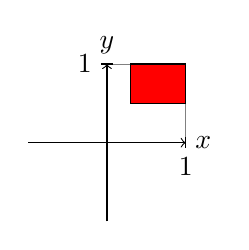
\begin{tikzpicture}

\draw (1.05cm,2pt) node[above]{};
 %  {$\displaystyle\int_0^{3/2} \!\!x^2\mathrm{d}x$};

\draw[style=help lines] (0,0) grid (1,1);
  % [step=0.25cm]      (1,2) grid +(1,1);

\draw[->] (-1,0) -- (1,0) node[right] {$x$};
\draw[->] (0,-1) -- (0,1) node[above] {$y$};

\foreach \x/\xtext in {1/1}
\draw[shift={(\x,0)}] (0pt,2pt) -- (0pt,-2pt) node[below] {$\xtext$};

\foreach \y/\ytext in {1/1}
\draw[shift={(0,\y)}] (2pt,0pt) -- (-2pt,0pt) node[left] {$\ytext$};

\draw[fill=red]  (0.3,0.5) -- (1,0.5) -- (1,1) -- (0.3,1) -- cycle;
\end{tikzpicture}
\end{center}

Now we calculate the probability of $A$.

We use the definition of the probability of a joint distribution function from
\cite{reading7}, and we apply the joint pdf of $X$, and $Y$ to this
defintition:

\begin{equation}
P \left( A \right) =
  \int_{0.5}^{1} \int_{0.3}^{1} \frac{3}{2}\left(x^2 + y^2 \right) \,dx\,dy.
\end{equation}

First we find the antiderivative of the pdf with respect to $x$:


\begin{equation}
P \left( A \right) =
  \int_{0.5}^{1} \frac{3}{2}\left(\frac{x^3}{3}
    + xy^2 \right) \bigg\rvert_{x=0.3}^{1}\,dy.
\end{equation}

And now we find the antiderivative of the pdf with respect to $y$:

\begin{equation}
P \left( A \right) =
  \frac{3}{2}\left(\frac{x^3y}{3}
    + x\frac{y^3}{3} \right) \bigg\rvert_{x=0.3}^{1} \bigg\rvert_{y=0.5}^{1}.
\end{equation}

We apply the distributive rule for multiplication to find that the equation
above is true if, and only if:

\begin{equation}
P \left( A \right) =
  \frac{1}{2}\left(x^3y
    + xy^3 \right) \bigg\rvert_{x=0.3}^{1} \bigg\rvert_{y=0.5}^{1}.
\end{equation}


Now we evaluate the antiderivatives over the intervals we specifiy in order
to compute the probability:

\begin{equation}
P \left( A \right) =
\left(  \frac{1}{2}\left(\left(1 \right)^3 \left(1 \right)
    + \left( 1 \right) \left(1 \right)^3 \right) \right) -
\left(  \frac{1}{2}\left(\left(0.3 \right)^3 \left(0.5 \right)
    + \left( 0.3 \right) \left(0.5 \right)^3 \right) \right).
\end{equation}

The equation above simplifies to:

\begin{equation}
P \left( A \right) =
1 -
\left(  \frac{1}{2}\left(\left(0.3 \right)^3 \left(0.5 \right)
    + \left( 0.3 \right) \left(0.5 \right)^3 \right) \right).
\end{equation}

We use a calculator to simplify the equation above further to:


\begin{equation}
P \left( A \right) =
1 -
\left(  \frac{1}{2} \left( 0.0135 +  0.0375 \right) \right).
\end{equation}

We use a calculator once more to find that $P\left( A \right) = 0.9745$.
Note: this differs from Orloff and Bloom's solution, however, it seems they
mistakenly use 4xy for the pdf of the joint distribution of $X$, and $Y$ in
\cite{slides7}

\subsection{Cumulative distribution function}

The cumulative distribution function (cdf), $F \left( x, y \right)$ of the pdf
for the joint distribution of $X$, and $Y$ the integral of its probability
density function $f\left(x, y \right)$ that Orloff and Bloom give for this
problem \cite{reading7}.

We replace vairables $x$, and $y$ with $u$, and $v$, so that we may use
$x$, and $Y$ as the upper limits of our integral.  Doing so yeilds a cdf in
terms of $x$, and $y$.


\begin{equation}
F\left( X, Y \right) = \int_0^y \int_0^x \frac{3}{2}\left( u^2
  + v^2 \right) \,du \,dv.
\end{equation}

Now we integrate with respect to $u$:

\begin{equation}
F\left( X, Y \right) = \int_0^y  \frac{3}{2}\left( \frac{u^3}{3}
  + uv^2 \right) \bigg\rvert_{u=0}^x \,dv.
\end{equation}

Next, we integrate with respect to v:

\begin{equation}
F\left( X, Y \right) =   \frac{3}{2}\left( \frac{uv^3}{3}
  + \frac{uv^3}{3} \right) \bigg\rvert_{u=0}^x \bigg\rvert_{v=0}^{y}.
\end{equation}

We evaluate the antiderivative at the limits of integration specified in the
equation above to obtain:


\begin{equation}
F\left( X, Y \right) =   \left( \frac{3}{2}\left( \frac{x^{3}y}{3}
  + \frac{xy^3}{3} \right)  \right) -
  \left( \frac{3}{2}\left( \frac{\left(0 \right) \left(0 \right)^3}{3}
  + \frac{\left(0 \right) \left( 0 \right) ^3}{3} \right)  \right)
\end{equation}

Finally we use the distributive rule for multiplication as well as some arithmetic
to simplify the equation above:

\begin{equation}
F\left( X, Y \right) =  \frac{1}{2}\left( x^{3}y + xy^3  \right)
\end{equation}

Note: this result disagrees with the one that Orloff and Bloom give in the
\cite{slides7Sol} for this question.  The reult Orloff and Bloom give is:
\begin{equation}
  F\left( X, Y \right) = \frac{x^3 y}{3} + \frac{x y^3}{3}.
\end{equation}

However, it is consistent with the function Orloff and Bloom use for
$F_{X} \left( x \right)$ in the fifth part of this problem in
\cite{slides7Sol}.

\subsection{Marginal PDF}

In order to find the marginal pdf $f_{X}\left(X \right)$ of
$f\left( x, y \right)$ we integrate out the variable $y$ \cite{reading7}.

\begin{equation}
  f\left( x, y \right) = \int_0^1 \frac{3}{2}\left( x^2 + y^2 \right) \,dy.
\end{equation}

We replace $f$ with its antiderivative, with a note to integrate over the
closed interval $\left[ 0 , 1\right]$:

\begin{equation}
  f_{X}\left(X \right) =  \frac{3}{2}\left( x^{2}y + \frac{y^3}{3} \right)
  \bigg\rvert_{y=0}^1.
\end{equation}

Now we replace $y$ in the equation above with the limits of integration:
\begin{equation}
  f_{X}\left(X \right) = \left( \frac{3}{2} \left( x^2 \left(1 \right)
      + \frac{ \left(1 \right)^3}{3}) \right) \right)
  - \left( \frac{3}{2} \left( x^2 \left(0 \right)
      + \frac{ \left(0 \right)^3}{3}) \right) \right)
\end{equation}

And we simplify the equation above to give the marginal probability in a more
agreeable form:

\begin{equation}
  f_{X}\left(X \right) = \frac{3}{2} \left( x^2 + \frac{1}{3} \right)
\end{equation}

Now that we have the marginal probability, we can answeer the second part of
the question, which is to find the marginal probability
$P \left( X < 0.5 \right)$.

$P \left( X < 0.5 \right)$ is the integral of $f_{X}\left(X \right)$ over the
interval $\left[0, 0.5 \right]$ \cite{reading7}.
\begin{equation}
  P \left( X < 0.5 \right) = \int_0^{0.5}
   \frac{3}{2} \left( x^2 + \frac{1}{3} \right) \,dx.
\end{equation}

We replace $f_{X}\left( X \right)$ with its antiderivative, evaluated over
the interval $\left[0, 0.5 \right]$:

\begin{equation}
  P \left( X < 0.5 \right) =
   \frac{3}{2} \left( \frac{x^3}{3} + \frac{x}{3} \right) \bigg\rvert_0^{0.5}.
\end{equation}

And we evaluate the antiderivative at the limits of integration:

\begin{equation}
  P \left( X < 0.5 \right) =
   \left( \frac{3}{2} \left( \frac{0.5^3}{3} + \frac{0.5}{3} \right) \right)
   - \left( \frac{3}{2} \left( \frac{0^3}{3} + \frac{0}{3} \right) \right)
\end{equation}

The equation above simplfies to:
\begin{equation}
  P \left( X < 0.5 \right) =
   \frac{3}{2} \left( \frac{1}{24} + \frac{1}{6} \right),
\end{equation}

which further simplifies to:

\begin{equation}
  P \left( X < 0.5 \right) = \frac{5}{16}.
\end{equation}


\subsection{Marginal cdf}

In this section we will do as Orloff and Bloom ask, and find the marginal
cumulative distribution function (cdf) $F_{X}\left(X \right)$, and
$P\left(X < 0.5 \right)$.

In \cite{reading7} Orloff and Bloom state that, ``If $X$ and $Y$ jointly take
values on $\left[a,b\right] \times \left[c, d \right]$, then
\begin{equation}
  F_{X}\left(X \right) = F\left(x, d\right),
  F_{Y} \left(Y \right) = F \left(b, y \right)."
\end{equation}

We must compute $P\left( X < 0.5 \right)$, so we use the marginal cdf
$F\left(x, 1 \right)$.

Previously in this problem, we found that the cdf for the joint distribution
we are dealing with is

\begin{equation}
F\left( X, Y \right) =  \frac{1}{2}\left( x^{3}y + xy^3  \right)
\end{equation}

Therefore

\begin{equation}\label{marginCdf}
  F\left(x, 1 \right) = \frac{1}{2}\left( x^{3} + x  \right)
\end{equation}

We use the definition of joint cdf from \cite{reading7} to write

\begin{equation}
P \left( X < 0.5 \right) = F\left(0.5, 1 \right).
\end{equation}

Now, we can replace the right hand side of the equation above with
the right hand side of equation \ref{marginCdf}, where we have
applied the value $0.5$ as the value for $x$ in the right hand
side of equation \ref{marginCdf}:

\begin{equation}
P \left( X < 0.5 \right) = \frac{1}{2}\left( 0.5^{3} + 0.5  \right).
\end{equation}

We use arithmetic to simplify the right hand side of the equation above to
find:

\begin{equation}
P \left( X < 0.5 \right) = \frac{5}{16}.
\end{equation}

\subsection{Cdf of discrete joint distribution}

In the last part of this question, Orloff and Bloom give a new, discrete
joint distribution for us to investigate.  They give us the following
table, that defines the joint distribution:


\begin{center}
  \begin{tabular}{ | c | c | c | c | c | c | c |}
    \hline
    $X/Y$ & 1  & 2  & 3  & 4  & 5  &  6    \\ \hline
    1     &  $\frac{1}{36}$  & $\frac{1}{36}$ & $\frac{1}{36}$ & $\frac{1}{36}$ & $\frac{1}{36}$ & $\frac{1}{36}$   \\ \hline
    2     &  $\frac{1}{36}$  & $\frac{1}{36}$ & $\frac{1}{36}$ & $\frac{1}{36}$ & $\frac{1}{36}$ & $\frac{1}{36}$   \\ \hline
    3     &  $\frac{1}{36}$  & $\frac{1}{36}$ & $\frac{1}{36}$ & $\frac{1}{36}$ & $\frac{1}{36}$ & $\frac{1}{36}$   \\ \hline
    4     &  $\frac{1}{36}$  & $\frac{1}{36}$ & $\frac{1}{36}$ & $\frac{1}{36}$ & $\frac{1}{36}$ & $\frac{1}{36}$   \\ \hline
    5     &  $\frac{1}{36}$  & $\frac{1}{36}$ & $\frac{1}{36}$ & $\frac{1}{36}$ & $\frac{1}{36}$ & $\frac{1}{36}$   \\ \hline
    6     &  $\frac{1}{36}$  & $\frac{1}{36}$ & $\frac{1}{36}$ & $\frac{1}{36}$ & $\frac{1}{36}$ & $\frac{1}{36}$   \\ \hline
  \end{tabular}
\end{center}

Note: the value in the $i,j^th$ entry in the table above is the probability that
$X=i$, and $Y=j$.

Orloff and Bloom ask us to find the joint cdf $F \left(3.5, 4 \right)$.

$F\left(3.5, 4 \right)$ is the sum of all probabilities where $X \leq 3.5$, and
$Y \leq 4$.

Therefore $F \left( 3.5, 4 \right)$ is the sum of the probabilities in the
shaded entries in the table below:


\begin{center}
  \begin{tabular}{ | c | c | c | c | c | c | c |}
    \hline
    $X/Y$ & 1  & 2  & 3  & 4  & 5  &  6    \\ \hline
    1     & \cellcolor{blue!25} $\frac{1}{36}$  & \cellcolor{blue!25} $\frac{1}{36}$ & \cellcolor{blue!25} $\frac{1}{36}$ & \cellcolor{blue!25} $\frac{1}{36}$ & $\frac{1}{36}$ & $\frac{1}{36}$   \\ \hline
    2     & \cellcolor{blue!25} $\frac{1}{36}$  & \cellcolor{blue!25} $\frac{1}{36}$ & \cellcolor{blue!25} $\frac{1}{36}$ & \cellcolor{blue!25} $\frac{1}{36}$ & $\frac{1}{36}$ & $\frac{1}{36}$   \\ \hline
    3     & \cellcolor{blue!25} $\frac{1}{36}$  & \cellcolor{blue!25} $\frac{1}{36}$ & \cellcolor{blue!25} $\frac{1}{36}$ & \cellcolor{blue!25} $\frac{1}{36}$ & $\frac{1}{36}$ & $\frac{1}{36}$   \\ \hline
    4     &  $\frac{1}{36}$  & $\frac{1}{36}$ & $\frac{1}{36}$ & $\frac{1}{36}$ & $\frac{1}{36}$ & $\frac{1}{36}$   \\ \hline
    5     &  $\frac{1}{36}$  & $\frac{1}{36}$ & $\frac{1}{36}$ & $\frac{1}{36}$ & $\frac{1}{36}$ & $\frac{1}{36}$   \\ \hline
    6     &  $\frac{1}{36}$  & $\frac{1}{36}$ & $\frac{1}{36}$ & $\frac{1}{36}$ & $\frac{1}{36}$ & $\frac{1}{36}$   \\ \hline
  \end{tabular}
\end{center}

There are 12 shaded entries in the table above, and they all have a value of
probability $\frac{1}{36}$.  Therefore the sum of the probabilities in all
the shaded squares is $ 12 \times \frac{1}{36} = \frac{1}{3}$.  Hence,
\begin{equation}
  P \left( 3.5, 4 \right) = \frac{1}{3}.
\end{equation}

We skip the next two questions on indpendence of discrete joint distributions because
we have already answered similar questions previously.

The next question from \cite{slides7} that we answer is one on independence
of continuous random variables of different probability mass functions.

Before we delve into the particulars of this problem, it behooves us to note the
definition of independence for continous jointly distributed random variables from
\cite{reading7}: $f \left(x, y \right)=f_{X}\left(x \right) f_{Y}\left(y \right)$.

Orloff and Bloom go on to state that jointly distributed random variables are
independent if we, ``\ldots can factor the joint pdf or cdf as the product of
a function of $X$ and a function of $y$."

For this problem, we are given 3 joint pdf's, and we assume that the joint
pdf's are defined over suitable regions such that the integrals over the
regions equal 1. The three joint pdf's are:
\begin{enumerate}
  \item $f \left( x, y \right) = 4x^2y^3$.
  \item $f \left( x, y \right) = \frac{1}{2} \left( x^3y + xy^3 \right)$.
  \item $f \left( x, y \right) = 6e^{-3x-2y}$
\end{enumerate}

We factor the first pdf.  Let $f\left(x \right) = 4x^2$,
$g\left(y \right)= 2y^3$.  Then
\begin{equation}
4x^2y^3 = f\left(x \right) g\left( y \right).
\end{equation}.

We can factor the first pdf as a function of $x$, and a function of $y$, so
$x$, and $y$ are independently  distributed with the first pdf.

\begin{lem}
$a^{x+y} = a^xa^y$

\begin{equation}
a^{x+y} = \underbrace{aaa \ldots a}_{\text{x+y a's}}.
\end{equation}

\text{We use the associative property of multiplication to state that the
above is true if and only if:}

\begin{equation}
a^{x+y} = \underbrace{aaa \ldots a}_{x\text{ }a\text{'s}}
\underbrace{aaa \ldots a}_{y\text{ }a\text{'s}}
\end{equation}

\begin{equation}
\underbrace{aaa \ldots a}_{x\text{ }a\text{'s}}
\underbrace{aaa \ldots a}_{y\text{ }a\text{'s}}
=a^xa^y.
\end{equation}

\text{Therefore}

\begin{equation}
a^{x+y} = a^xa^y.
\end{equation}
\end{lem}

We factor the third pdf. Let $f\left(x \right)=e^{-3x}$, and let
$g\left(y, \right) = e^{-2y}$.

The lemma above implies that $e^{-3x} e^{-2y}=e^{-3x-2y}$.  Therefore we can
factor $e^{-3x-2y}=f\left(x \right) g\left(y \right)$.  Hence $x$ and $y$ are
independently distributed in the distribution with the third pdf.

If random variables $X$ and $Y$ follow the joint distribution with the second
pdf, then they cannot be indpendent. We factor the pdf:
\begin{equation}
  \frac{1}{2}\left(x^3y + xy^3 \right) = \frac{1}{2}\left(xy \right)\left(x^2 + y^2 \right)
  = \frac{1}{2}\left(xy \right)\left(x +y \right)\left( x - y \right).
\end{equation}


Any factorization of $f\left(x, y\right)$ would involve
some product of the factors of $f\left(x, y\right)$ that
we find above.  However, each of these factors involves
$x$, and $y$.

Therefore we cannot factor $f\left( x, y \right)$ as
the product of two functions $f\left(x \right)$, and
$g\left(y \right)$.

\section{Covariance of coin flips}

Orloff and Bloom give us the following problem:
We flip a fair coin 3 times.  We let $X$ be the
number of heads in the first 2 flips, and we
let $Y$ be the number of heads in the last two flips.

The problem Orloff and Bloom give us is to calculate
the covariance of $X$ and $Y$.

The expected value $E\left( X \right)$, of $X$
is:
\begin{equation}
E\left(X \right)  =
  \frac{1}{4}\times 0 + \frac{1}{2} \times 1 + \frac{1}{4} times 2 = 1.
\end{equation}

Similarly the expected value $E\left( Y \right)$ of $Y$ is also 1.

We use the technique from \cite{reading7b} and write $X$ and $Y$
as the sum of independent Bernoulli random variables
$X_1$, $X_2$, and $X_3$, where $X_1$ is the outcome
of the Bernoulli trial of flipping the coin for the
first time, and so on.


We use the property of covariance from \cite{reading7b}

\begin{equation}\label{covarForm}
\text{Cov}\left(X_1 + X_2, Y \right)
 = \text{Cov}\left(X_1, Y \right) + \text{Cov}\left(X_2, Y \right).
\end{equation}

We substitute $Y=X_2 + X_3$

\begin{equation}
\text{Cov}\left(X_1 + X_2, X_2 + X_3 \right)
 = \text{Cov}\left(X_1, X_2 + X_3 \right) + \text{Cov}\left(X_2, X_2 + X_3 \right).
\end{equation}

Now we use the identity:
\begin{equation}
\text{Cov}\left(X, Y \right) = E\left(XY\right) -\mu_X\mu_Y.
\end{equation}

We use the commutative property of multiplication:
\begin{equation}
\text{Cov}\left(X, Y \right) = E\left(YX\right) -\mu_Y\mu_X.
\end{equation}

Therefore
\begin{equation}
\text{Cov}\left(X, Y \right) = \text{Cov}\left(Y, X \right).
\end{equation}

We apply the identity above to equation \ref{covarForm} to get:

\begin{equation}
\text{Cov}\left(X_1 + X_2, X_2 + X_3 \right)
  =\text{Cov}\left(X_2 + X_3, X_1 \right) + \text{Cov}\left(X_2 + X_3, X_2  \right).
\end{equation}

Now we can apply equation \ref{covarForm} again to the equation
above:

\begin{equation}
\text{Cov}\left(X_1 + X_2, X_2 + X_3 \right)
  =\text{Cov}\left(X_2, X_1 \right) + \text{Cov}\left(X_2, X_2  \right) +
   \text{Cov}\left(X_3, X_1 \right) + \text{Cov}\left(X_3, X_2  \right)
\end{equation}

The Bernoulli trials $X_1$, and $X_3$; and $X_1$ and $X_2$;
and $X_2$, and $X_3$ are independent events. Therefore:
$\text{Cov}\left(X_2, X_1 \right) = 0$,
$\text{Cov}\left(X_3, X_1 \right) = 0$, and
$\text{Cov}\left(X_3, X_2  \right) = 0$.

Therefore in order to compute $\text{Cov}\left(X_1 + X_2, X_2 + X_3 \right)$,
We need only compute $\text{Cov}\left(X_2, X_2 \right)$.

In \cite{reading7b} Orloff and Bloom state that
$\text{Cov}\left(X, X\right) = \text{Var}\left(X\right)$.

$X_2$ is the toss of a fair coin, so it has expected value
$0\times\frac{1}{2} + 1 \times\frac{1}{2} = \frac{1}{2}$,
and variance
$\frac{1}{2}\left(0 - \frac{1}{2}\right)^2 + \frac{1}{2}\left(1-\frac{1}{2}\right)^2 = \frac{1}{4}$.

Therefore

\begin{equation}
\text{Cov}\left(X_1 + X_2, X_2 + X_3 \right)
  = \frac{1}{4}.
\end{equation}

We defined $X=X_1+X2$, and $Y=X_2+X_3$, therefore
\begin{equation}
\text{Cov}\left(X, Y \right)
  = \frac{1}{4}.
\end{equation}

\section{Correlation and Covariance of variables}
\subsection{Covariance}

Orloff and Bloom ask us to consider
flipping a fair coin $2n + 1$ times.
They define the random variable $X$
to be the number of heads in the first 
$n+1$ coim flips, and they define the
random variable $Y$ to be the number of
heads in the last $n+1$ flips. Orloff
and Bloom then ask us to find the 
covariavariance Cov$\left(X,Y \right)$.

We use reasoning similar to the problem
Orloff and Bloom gave us regarding 3 coin
flips. We look at that problem as the case
where $n=3$.

Each coin flip is one independent Bernoulli
trial with probability $\frac{1}{2}$.

We define a set of random variables first we define the abstract random
variable $X_i$.  We call $X_i$ abstract because we have not given a particular
value for $i$.
\begin{equation}
 X_i = \begin{cases} 
 	1 & \mbox{We flip the coin heads up on the $i^{th}$ toss.} \\
 	0 & \mbox{We filp the coin tails up on the $i^{th}$ toss.} \\
 	\end{cases}
\end{equation}

Now we can define $X$ and $Y$ in terms of the $X_i$. 
\begin{equation}
X = \sum_{i=1}^{n+1} X_i.
\end{equation}

\begin{equation}
Y = \sum_{i=n}^{2n+1} X_i.
\end{equation}

Therefore
\begin{equation}
\text{Cov}\left( X, Y \right) = 
  \text{Cov}\left(\sum_{i=1}^{n+1} X_i, \sum_{j=n+1}^{2n} X_j \right).
\end{equation}

We use equation \ref{covarForm} repeatedly to justify the statement that
the previous equation is true if, and only if:

\begin{equation}
\text{Cov}\left( X, Y \right) = 
  \sum_{i=1}^{n+1} \text{Cov}\left(X_i, \sum_{j=n+1}^{2n} X_j \right).
\end{equation}

Now, since Cov$\left(X, Y \right) = \text{Cov}\left(Y, X \right)$,

\begin{equation}
\text{Cov}\left( X, Y \right) = 
  \sum_{i=1}^{n+1} \text{Cov}\left(\sum_{j=n+1}^{2n} X_j , X_i \right).
\end{equation}

And we apply equation \ref{covarForm} to the previous equation to obtain:

\begin{equation}\label{doubleSum}
\text{Cov}\left( X, Y \right) = 
  \sum_{i=1}^{n+1} \sum_{j=n+1}^{2n}\text{Cov}\left(X_j , X_i \right).
\end{equation}

Each toss of a fair coin is an independent Bernoulli trial, so if $i \neq j$,
then Cov$\left(X_i, X_j\right) = 0$ \cite{reading7b}.

Therefore the only term in equation \ref{doubleSum} that is not 0 is
Cov$\left(X_{n+1}, X_{n+1} \right)$.

We found in the previous problem involving three flips of a fair coin
that the Covariance is $\frac{1}{4}$.

Therefore 

\begin{equation}
\text{Cov}\left( X, Y \right) = \frac{1}{4}.
\end{equation}

\subsection{Correlation}

Orloff and Bloom define correlation in \cite{reading7b}. We denote correlation
with the Greek letter $\rho$.


\begin{equation}
\rho = frac{\text{Cov} \left(X, Y \right) } {\sigma_X \sigma_Y}.
\end{equation}

$X$ and $X$ are both the number of heads in $n+1$ coin tosses, so their
standard deviation will be the same.

Therefore we will determine $\sigma_X$, and we will also know what $\sigma_Y$
is.

Let $X_i$ have the same definition that it has in the previous section.

Then  we use the definition of variance of a discrete random variable 
\cite{reading5a} to write:

\begin{equation}
\text{Var}\left(X_i\right) = p\left(0 \right) \left(0-\mu_{X_i}\right)^2
     + p\left(1 \right) \left(1-\mu_{X_i}\right)^2.
\end{equation}

$X_i$ is equal to $1$ if we toss a fair coin heads up, and $0$ otherwis,
so $\mu_{X_i} = \frac{1}{2}$, and 
$p\left(0\right) = p\left(1 \right) = \frac{1}{2}$.

Therefore 

\begin{equation}
\text{Var}\left(X_i\right) = \frac{1}{2} \left(0-\frac{1}{2} \right)^2
     + \frac{1}{2} \left(1-\frac{1}{2} \right)^2.
\end{equation}

We do the arithmetic on the right hand side of the previous equation to
find:

\begin{equation}
\text{Var}\left(X_i\right) = \frac{1}{4}.
\end{equation}


Now we repeatedly use the first property of variance from \cite{reading5a}
and the equation above to write:

\begin{equation}
\text{Var}\left( \sum_{i=1}^{n+1} X_i \right) = 
     \sum_{i=1}^{n+1} \text{Var}\left(X_i \right).
\end{equation}

Since Var$\left(X_i \right) = \frac{1}{4}$, 

\begin{equation}
\text{Var}\left( \sum_{i=1}^{n+1} X_i \right) = 
     \sum_{i=1}^{n+1} \frac{1}{4}.
\end{equation}

Now we evaluate the sum above to find:
\begin{equation}
\text{Var}\left( \sum_{i=1}^{n+1} X_i \right) = 
     \frac{n+1}{4}.
\end{equation}

Since $X$ and $Y$ are both the number of heads in $n+1$ tosses of a fair coin,
Var$\left(X \right) = \text{Var}\left(Y \right) = \frac{n+1}{4}$, and
$\sigma_X = \sigma_Y = \sqrt{\frac{n+1}{4}} = \frac{\sqrt{n+1}}{2}$.

Therefore

\begin{equation}
\rho = \frac{ \frac{1}{4} }{ \frac{\sqrt{n+1}}{2}\frac{\sqrt{n+1}}{2}}
\end{equation}

The previous equation simplifies to :

\begin{equation}
\rho = n+1.
\end{equation}


\printbibliography{}


\end{document}
